\documentclass[openright]{memoir}

\usepackage{amsmath}
\usepackage{graphicx}
\usepackage{xcolor}
\usepackage{tikz}
\usetikzlibrary{calc}
\usepackage{blindtext}

\newlength{\mylength}

% set page size
\setstocksize{275mm}{215mm}
\settrimmedsize{\stockheight}{\stockwidth}{*}

% set left and right typeblock margins
\setlrmarginsandblock{1.94in}{0.63in}{*}
% set top and bottom typeblock margins
\setulmarginsandblock{0.78in}{*}{1}
% set margin note margins
\setmarginnotes{0.15in}{1.22in}{\onelineskip}

% margin and side notes always on left side
\marginparmargin{left}
\sideparmargin{left}

\checkandfixthelayout

\setlength{\evensidemargin}{\oddsidemargin}

% force side notes be left-aligned
\renewcommand{\sideparform}{\flushleft}

% create memst pagestyle
\makepagestyle{memst}

\newlength{\marginpartotal}
\setlength{\marginpartotal}{\marginparsep}
\addtolength{\marginpartotal}{\marginparwidth}

% define header width
\setlength{\headwidth}{\textwidth}
\addtolength{\headwidth}{\marginparsep}
\addtolength{\headwidth}{\marginparwidth}
% set header width
\makerunningwidth{memst}{\headwidth}
% right align
\makeheadposition{memst}{flushright}{flushright}{}{}

\renewcommand{\chaptermark}[1]{\markboth{#1}{}}
\makeevenhead{memst}{%
    \textsf{%
        \textbf{\thepage}%
        \hspace{0.14in}%
        \MakeUppercase\chaptername~\thechapter~|~\leftmark%
    }
}{}{}

\definecolor{oddheadcolor}{RGB}{12, 12, 106}
\renewcommand{\sectionmark}[1]{\markright{#1}}
\makeoddhead{memst}{}{}{\textsf{
    \textcolor{oddheadcolor}{%
        SECTION~\thesection~|~\rightmark%
    }%
    \hspace{0.17in}%
    \textbf{\thepage}%
}}

% section heading style
\definecolor{sectionheadingcolor}{RGB}{163, 156, 112}
\newcommand{\mysecheadstyle}[1]{%
    \color{sectionheadingcolor}\LARGE\scshape#1%
    \vspace{-9pt}\hspace{-\marginpartotal}\hspace{-14.5pt}%
    \rule{\headwidth}{\normalrulethickness}%
}

\makeatletter
\def\@seccntformat#1{\csname #1@cntformat\endcsname}
\newcommand{\section@cntformat}{%
    \color{oddheadcolor}\bfseries\LARGE\thesection\quad%
}
\makeatother

\setsecindent{-\marginpartotal}
\setsecheadstyle{\mysecheadstyle}

% subsection heading style
\setsecnumdepth{subsection}

\newcommand{\mysubsecheadstyle}[1]{%
    \Large\bfseries\textsf{#1}%
}

\makeatletter
\newcommand{\subsection@cntformat}{%
    \Large\bfseries\textsf{\S}~%
}
\makeatother

\setsubsecindent{-15pt}
\setsubsecheadstyle{\mysubsecheadstyle}

% create chapter toc for memst chapterstyle
\newcounter{tocmarker}
\renewcommand\mempreaddchaptertotochook{\cftinserthook{toc}{end-\thetocmarker}}
\renewcommand\mempreaddparttotochook {\cftinserthook{toc}{end-\thetocmarker}}
\renewcommand\mempreaddbooktotochook {\cftinserthook{toc}{end-\thetocmarker}}
\renewcommand\mempreaddapppagetotochook{\cftinserthook{toc}{end-\thetocmarker}}
% start marker
\renewcommand\mempostaddchaptertotochook{%
    \stepcounter{tocmarker}\cftinserthook{toc}{start-\thetocmarker}
}
\let\normalchangetocdepth\changetocdepth % for later
\makeatletter
\newcommand\chaptertoc{
    % make changes local, remember counters a global
    \begingroup
        \renewcommand\markboth[2]{}
        \sffamily
        % store current value, to be restored later
        \setcounter{@memmarkcntra}{\value{tocdepth}}
        % when ever \settocdepth is used, it adds the new value to the
        % ToC data. This cause problems when we want to disable all
        % entries. Luckily the data is added via a special macro, we we
        % redefine it, remember we stored the original value earlier.
        \let\changetocdepth\@gobble
        % disable all entries (using our copy from above)
        \normalchangetocdepth{-10}
        % enable toc data within our block, we go as far as subsubsection
        \cftinsertcode{start-\thetocmarker}{\normalchangetocdepth{1}}
        % when the block is done, disable the remaining
        \cftinsertcode{end-\thetocmarker}{\normalchangetocdepth{-10}}
        % remove the spacing above the toc title
        \let\tocheadstart\relax
        % remove the toc title itself
        \let\printtoctitle\@gobble
        % remove space below title
        \let\aftertoctitle\relax
        % reformat TOC entries:
        \setlength{\cftsectionindent}{0pt}
        \setlength{\cftsubsectionindent}{\cftsectionnumwidth}
        \setlength{\cftsubsubsectionindent}{\cftsubsectionindent}
        \addtolength{\cftsubsubsectionindent}{\cftsubsectionnumwidth}
        \renewcommand\cftsectionfont{\small}
        \renewcommand\cftsectionpagefont{\small}
        \renewcommand\cftsubsectionfont{\small}
        \renewcommand\cftsubsectionpagefont{\small}
        \renewcommand\cftsubsubsectionfont{\small}
        \renewcommand\cftsubsubsectionpagefont{\small}
        % no dots before page number
        \renewcommand\cftdot{}
        % disable page number for sections
        \cftpagenumbersoff{section}
        % include the actual ToC data
        \tableofcontents*
    \endgroup
    % restore tocdepth
    \setcounter{tocdepth}{\value{@memmarkcntra}}
    % to indent or not after the chapter toc
    \m@mindentafterchapter
    % space between chapter toc and text
    \par\bigskip
    % handles indentation after the macro
    \@afterheading
}
\makeatother

% create memst chapterstyle
\definecolor{chapterstylenorthwest}{RGB}{63, 124, 148}
\definecolor{chapterstylenortheast}{RGB}{89, 0, 89}
\newlength{\cns}
\setlength{\cns}{6.8pt}

\makechapterstyle{memst}{
    \renewcommand{\chapternamenum}{}
    \renewcommand{\printchaptername}{
        \begin{tikzpicture}[remember picture, overlay]
            % top left tirquoise rectangle
            \fill[chapterstylenorthwest]%
                (current page.north west) rectangle ($(current page.north west)+(3.09in, -0.78in)$);
            \node[anchor=north west, inner sep=0pt, xshift=3.09in] at (current page.north west) {%
            % main picture
                \includegraphics[width=4.63in, height=3.14in]{chapter-\thechapter-title.jpg}%
            };
            % top right purple rectangle
            \fill[chapterstylenortheast]%
                ($(current page.north west)+(7.72in, 0in)$) rectangle ($(current page.north east)+(0in, -3.14in)$);
            % CHAPTER letters in white color
            \node[%
                anchor=north west, inner sep=0pt, rotate=90%
            ] at ($(current page.north west)+(8.01in, -2.67in)$) {%
                \color{white}\huge\textsf{
                    C\hspace{\cns}H\hspace{\cns}A\hspace{\cns}P\hspace{\cns}T\hspace{\cns}E\hspace{\cns}R\hspace{\cns}%
                }%
            };
            % horizontal white line between CHAPTER and chapter number
            \draw[line width=0.4pt, color=white] ($(current page.north east)+(-0.48in, -0.85in)$)%
                -- ($(current page.north east)+(-0.24in, -0.85in)$);
        \end{tikzpicture}
    }
    \renewcommand{\printchapternum}{
        % page number in white color
        \begin{tikzpicture}[remember picture, overlay]
            \node[xshift=-0.36in, yshift=-0.47in] at (current page.north east) {%
                \color{white}\HUGE\textsf{\thechapter}%
            };
        \end{tikzpicture}
    }
    \renewcommand{\printchaptertitle}[1]{
        \begin{tikzpicture}[remember picture, overlay]
            % chapter title
            \node[anchor=north west, inner sep=0pt, xshift=0.6in, yshift=-3.85in] at (current page.north west) {%
                \color{oddheadcolor}\HUGE\textsf{##1}%
            };
            % line under chapter title
            \draw[line width=0.4pt, color=oddheadcolor] ($(current page.north west)+(0.58in, -4.17in)$)%
                -- ($(current page.north east)+(-0.62in, -4.17in)$);
        \end{tikzpicture}
    }
}

% define completechapterpage command
\newcommand{\completechapterpage}[1]{
    \begin{tikzpicture}[remember picture, overlay]
        % chapter table of contents
        \node[anchor=north west, inner sep=0pt, xshift=0.58in, yshift=-4.92in] at (current page.north west) {%
            \begin{minipage}{3.4in}
                \chaptertoc
            \end{minipage}
        };
        % chapter introduction
        \node[%
            anchor=north west, inner sep=0pt, text width=3.69in, xshift=4.14in, yshift=-4.92in%
        ] at (current page.north west) {#1};
    \end{tikzpicture}
    \clearpage
}

% define frontps pagestyle
\makepagestyle{frontps}

\newlength{\frontpsfootwidth}
\setlength{\frontpsfootwidth}{\paperwidth}
\addtolength{\frontpsfootwidth}{-2\spinemargin}
\makerunningwidth{frontps}{\frontpsfootwidth}
\makeheadposition{frontps}{}{}{flushleft}{flushleft}

\makeevenhead{frontps}{}{}{}
\makeoddhead{frontps}{}{}{}
\makeevenfoot{frontps}{}{\roman{page}}{}
\makeoddfoot{frontps}{}{\roman{page}}{}

\begin{document}

\frontmatter

\pagestyle{frontps}
\chapterstyle{default}
\calccentering{\mylength}
\begin{adjustwidth*}{\mylength}{-\mylength}
\tableofcontents*\thispagestyle{frontps}
\newpage
\listoffigures\thispagestyle{frontps}
\end{adjustwidth*}

\mainmatter

\pagestyle{memst}
\chapterstyle{memst}
\aliaspagestyle{chapter}{empty}

\chapter{Fundamentals}
\completechapterpage{Perhaps the most useful idea for modeling the real world is
the concept of \emph{function}. Let's look at an example. If a rock climber
drops a stone from a high cliff, we know that the stone will fall. But this
general description doesn't help us figure out when the stone will hit the
ground. To find out, we need a \emph{rule} that relates the distance $d$ the
stone falls to the time it has been falling. Galileo was the first to discover
the rule: In $t$ seconds the stone falls $16t^2$ feet. This
“rule” is called a \emph{function}; we write this function as $d(t) = 16t^2$.
Using this function model, we can \emph{predict} when the stone will hit the
ground. In this chapter we study properties of functions and how function models
can help us to get precise information about the thing or process being
modeled.}

\section{What is a Function?}

A function is a rule.\sidepar{\itshape We have previously used letters to stand
for numbers. Here we do something quite different: We use letters to represent
rules.}
To talk about a function, we need to give it a name.
We will use letters such as $f$, $g$, $h$, $\ldots$ to represent
functions.

\Blindtext[3]

\section{Graphs of Functions}

The graph of a function\marginpar{\raisebox{-\height}{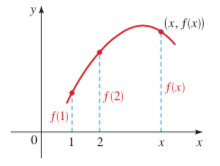
\includegraphics[width=\marginparwidth]{figure2}}}
$f$ gives a picture of the behavior or “life history” of the function. We can
read the value of $f(x)$ from the graph as being the height of the graph above
the point $x$.

\Blindtext[2]

\section{Getting Information from the Graph of a Function}

\blindmathpaper

\section{Average Rate of Change of a Function}

\subsection{Average Rate of Change}

We are all familiar with the concept of speed: If you drive a distance of 120
miles in 2 hours, then your average speed, or rate of travel, is
$\frac{120 mi}{2 h} = 􏱁 60 mi/h$. Now suppose you
take a car trip and record the distance that you travel every few minutes. The
distance $s$ you have traveled is a function of the time $t$:
\[
s(t) = \text{total distance traveled at time } t
\]
We graph the function $s$ as shown in \fref{fig:1}. The graph shows that you
have traveled a total of 50 miles after 1 hour, 75 miles after 2 hours, 140
miles after 3 hours, and so on. To find your average speed between any two
points on the trip, we divide the distance traveled by the time elapsed.

\begin{figure}
\centering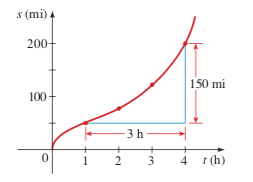
\includegraphics[scale=.6]{figure1}
\caption{Average speed}\label{fig:1}
\end{figure}

\Blindtext

\chapter{Polynomial and Rational Functions}
\completechapterpage{Functions defined by polynomial expressions
are called polynomial functions.
The graphs of polynomial functions can have many peaks and valleys;
this makes them suitable models for many real-world situations.
For example, a factory owner notices that if she increases the number
of workers, productivity increases, but if there are too many workers,
productivity begins to decrease.
This situations is modeled by a polynomial function of degree 2 (a quadratic function).
As another example, when a volleyball is hit, it goes up and then
down, following a path that is also modeled by a quadratic function.
The graphs of polynomial functions are smooth curves that are used
in designing many things. For example, sailboat designer put together
portions of the graphis of different cubic functions (called cubic splines) to
make the curves of the hull of a sailboat.}


\section{Quadratic Functions and Models}

\blindtext

\section{Polynomial Functions and Their Graphs}

\blindmathpaper

\section{Dividing Polynomials}

\Blindtext

\section{Real Zeros of Polynomials}

\blindmathpaper

\section{Complex Numbers}

\blindtext
\Blindlist{enumerate}

\chapter{Exponential and Logarithmic Functions}
\completechapterpage{\blindtext[1]}

\section{Exponential Functions}

\blindmathpaper

\section{The Natural Exponential Function}

\Blindlist{description}

\section{Logarithmic Functions}

\Blindlist{itemize}

\section{Laws of Logarithms}

\Blindtext

\end{document}